% Generated from artifacts/research/mlp/analysis/{findings.md,summary.csv,paired_tests.csv,
% reliability_summary.csv,stability_summary.csv,ablation_a_summary.csv,
% ablation_a_gate_statistics.csv}, artifacts/research/mlp/benchmark/benchmark_results.csv,
% and (Section~\ref{sec:legacy}) artifacts/research/mlp_legacy_sources/.
% Every number below is traceable to those files (see research/results_analysis.md).

\textbf{Executed experiments.} The main study follows the research protocol
(\texttt{configs/mlp.yaml}): 30-epoch dense, gated ($\lambda=0$) and Slimming sources
for five seeds, 5 fine-tuning epochs for every compact model, and ablations A and C on
three seeds. All of it ran on CPU (23\,h). The sources reach $60.06\pm0.17$ (dense),
$60.14\pm0.16$ (gated) and $59.51\pm0.08\%$ (Slimming) test accuracy.
Section~\ref{sec:legacy} summarizes the earlier verification on the original 5-epoch
checkpoints. The VGG-16-BN study was not executed (no GPU).

\subsection{Pruning accuracy (RQ1, RQ2)}
Table~\ref{tab:mlp_main} and Fig.~\ref{fig:acc} show test accuracy after fine-tuning.
The existing gate-in score gives the lowest accuracy of all criteria at every ratio:
$58.26$, $56.29$ and $53.58\%$ at $20$, $40$ and $60\%$ removal, against $59.98$, $59.22$
and $57.95\%$ for random selection on the same source. Before fine-tuning the gap is
larger: $44.8$/$30.5$/$18.9\%$ for gate-in against $57.4$/$46.9$/$24.0\%$ for random
(Fig.~\ref{fig:recovery}). All 15 alternative criteria beat gate-in on all five seeds at
every ratio, by $+1.2$ to $+2.2$\,pp at $20\%$, $+2.9$ to $+3.7$\,pp at $40\%$ and
$+4.4$ to $+5.3$\,pp at $60\%$. The Holm-corrected paired $t$-test supports every one of
these 45 differences at $p<0.05$ (largest adjusted $p$: $0.0046$ at $20\%$). With five
pairs the exact Wilcoxon test cannot fall below $p=0.0625$ and reaches that floor for
every comparison; Shapiro--Wilk rejects normality of the differences for 4 of the 45
comparisons, all at $20\%$.

The separately implemented gate variants, mean outgoing gate (V1) and the combined score
(V2), reach the level of the magnitude criteria (e.g.\ $58.72$ and $58.66\%$ at $60\%$,
against $58.82\%$ for $\ell_1$ and Taylor). This is consistent with
Section~\ref{sec:analysis}: BN cancels a neuron's incoming-gate level but not its outgoing
gates. In layer~1 the gate-in scores have a within-layer coefficient of variation of
$\approx9\times10^{-4}$ on every seed, against $0.11$--$0.12$ for $\ell_1$ and $0.57$--$0.59$
for Taylor. We did not test differences among the other criteria and claim no ranking
among them. Descriptively, Taylor, $\ell_1$, $\ell_2$ and $|\gamma|$ lie within
$0.35$\,pp of each other, and at $20\%$ Taylor and $\ell_1$ are within $0.1$\,pp of the
unpruned + fine-tuning control ($60.46\%$). The same criterion on the dense source gives
nearly identical accuracy ($\ell_1$ at $60\%$: $58.78$ dense vs.\ $58.82\%$ gated), so
gate training at $\lambda=0$ did not make the network more prunable. Network Slimming
retains the most accuracy before fine-tuning at $40$--$60\%$, but after fine-tuning it ends
$0.25$--$1.0$\,pp below Taylor on the gated source; its own source is $0.6$\,pp weaker, so
criterion and source are confounded. Global allocation for Slimming yields different,
smaller architectures ($-32$/$-59$/$-78\%$ parameters) and is not an equal-cost comparison.

\begin{table}[t]
\centering
\caption{\texttt{mlp}: test accuracy (\%, mean $\pm$ sample SD over 5 seeds) after 5 fine-tuning epoch(s). Criteria score the gated source except Net. Slimming (own training objective); identical compact architectures per column.}
\label{tab:mlp_main}
\footnotesize
\begin{tabular}{lccc}
\toprule
Method & 20\% units removed & 40\% units removed & 60\% units removed \\
\midrule
Gate-in (existing) & 58.26 $\pm$ 0.24 & 56.29 $\pm$ 0.16 & 53.58 $\pm$ 0.28 \\
Taylor & 60.43 $\pm$ 0.24 & 59.98 $\pm$ 0.13 & 58.82 $\pm$ 0.33 \\
Activation & 60.17 $\pm$ 0.40 & 59.60 $\pm$ 0.41 & 58.37 $\pm$ 0.18 \\
L1 in+out & 60.39 $\pm$ 0.09 & 59.96 $\pm$ 0.26 & 58.82 $\pm$ 0.21 \\
L2 in+out & 60.26 $\pm$ 0.42 & 60.04 $\pm$ 0.14 & 58.63 $\pm$ 0.42 \\
Net. Slimming & 59.41 $\pm$ 0.23 & 59.27 $\pm$ 0.29 & 58.57 $\pm$ 0.19 \\
Gate-combined (V2) & 60.26 $\pm$ 0.17 & 59.68 $\pm$ 0.28 & 58.66 $\pm$ 0.21 \\
Gate-out (V1) & 60.16 $\pm$ 0.21 & 59.87 $\pm$ 0.21 & 58.72 $\pm$ 0.08 \\
Random & 59.98 $\pm$ 0.24 & 59.22 $\pm$ 0.22 & 57.95 $\pm$ 0.07 \\
\midrule
Unpruned gated + FT & \multicolumn{3}{c}{60.46 $\pm$ 0.20} \\
Unpruned dense + FT & \multicolumn{3}{c}{60.27 $\pm$ 0.23} \\
Unpruned slimming + FT & \multicolumn{3}{c}{59.76 $\pm$ 0.24} \\
\bottomrule
\end{tabular}
\end{table}

\begin{figure}[t]
\centering
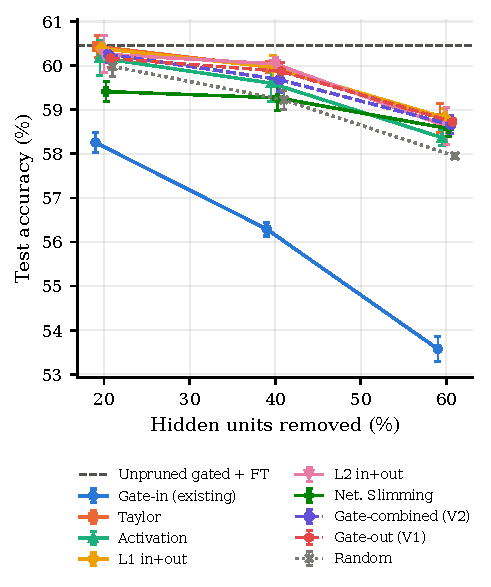
\includegraphics[width=0.85\columnwidth]{mlp/fig_accuracy_vs_ratio.pdf}
\caption{Test accuracy after five fine-tuning epochs (mean $\pm$ SD, 5 seeds; markers
offset horizontally for legibility). Dashed: unpruned gated model with the same
fine-tuning budget.}
\label{fig:acc}
\end{figure}

\begin{figure}[t]
\centering
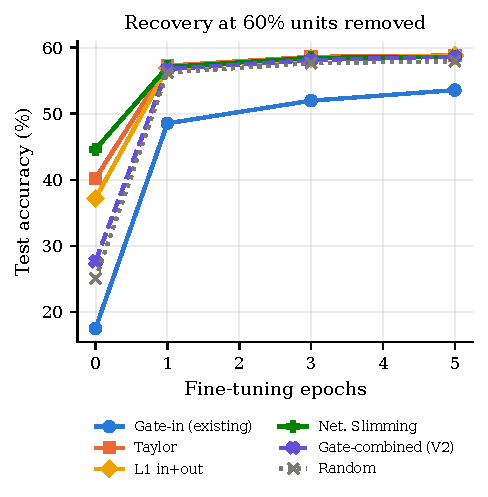
\includegraphics[width=0.85\columnwidth]{mlp/fig_finetune_recovery.pdf}
\caption{Accuracy immediately after pruning (dotted) and after fine-tuning (solid), mean
over 5 seeds.}
\label{fig:recovery}
\end{figure}

\subsection{Agreement with single-unit removal damage (RQ5)}
Fig.~\ref{fig:rel} reports Spearman's $\rho$ between each score and the validation-loss
increase caused by removing one unit (64 units per layer, 3 layers, 5 seeds). Gate-in is
the lowest criterion and negatively correlated with damage ($\rho=-0.161\pm0.088$; per
layer $-0.08$, $-0.21$, $-0.19$), below random ($-0.043\pm0.077$). On the dense and gated
sources every correlation is weak ($|\rho|\le0.17$): removing one unit changes the loss by
$1.7\times10^{-4}$ nats on average, and $23$--$24\%$ of removals \emph{decrease} it. On
the Slimming source all non-random criteria correlate more strongly with damage
($0.22$--$0.32$), and fewer removals reduce the loss ($20\%$). Taylor and activation scores
are stable under resampling of the calibration set (Spearman $0.96$--$0.99$ between two
disjoint subsets), so their weak reliability is not estimation noise. Single-unit damage
is not additive over the large groups removed in practice, so RQ5 and RQ1 measure
different properties.

\begin{figure}[t]
\centering
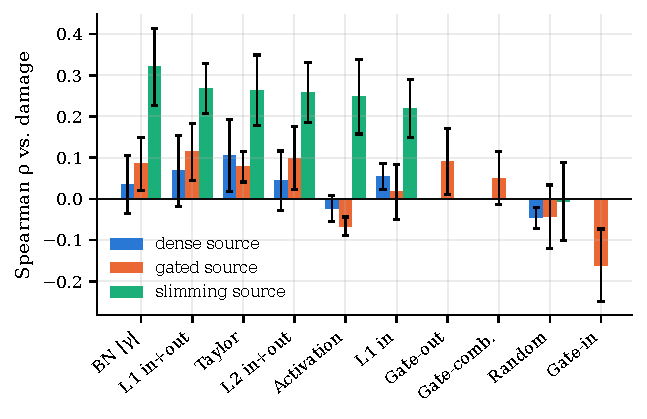
\includegraphics[width=\columnwidth]{mlp/fig_reliability_spearman.pdf}
\caption{Spearman $\rho$ between importance score and single-unit removal damage (mean
over layers, then mean $\pm$ SD over 5 seeds). Gate criteria exist only for the gated
source.}
\label{fig:rel}
\end{figure}

\subsection{Measured efficiency (RQ4)}
Uniform allocation gives identical architectures for every criterion. Deployable
parameters fall from $8.93$\,M to $6.73$, $4.73$ and $2.95$\,M ($-24.6$, $-47.0$,
$-67.0\%$), with MACs and serialized size reduced proportionally; these are physical
reductions of dense tensors. Median single-thread CPU latency at batch size 64 falls from
$11.95$\,ms to $9.47$, $6.56$ and $4.43$\,ms. Batch-1 latency also fell in this run
($1.17\to0.84$, $0.52$, $0.32$\,ms), but in the verification experiment the $20\%$ model
measured slower than dense at batch size 1, so we claim speed-ups only at batch size 64.
The gated model as trained, which recomputes $W\odot\sigma(S)$ in every forward pass,
takes $12.98$\,ms at batch size 1 ($\approx11\times$ the dense model); gates must be
folded into the weights before deployment. No GPU measurements were made.

\subsection{Verification on the original checkpoints}\label{sec:legacy}
Before the main study we evaluated the committed 5-epoch checkpoints of the existing
repository (3 seeds, $\approx52\%$ test accuracy, 1 fine-tuning epoch, each seed on its
own original split). The outcome was the same: gate-in was below random at every ratio
($47.05$ vs.\ $50.14\%$ at $60\%$), all 13 alternatives beat it on every seed, and its
scores were negatively correlated with removal damage ($\rho=-0.119\pm0.039$). Full tables
are in \texttt{research/results\_analysis.md}, Part~II.

\section{Ablation Studies}\label{sec:ablation}
The framework defines five ablations: A, gate penalty strength; B, gate aggregation
(incoming, outgoing, combined); C, fine-tuning budget; D, pruning ratio; E, seeds. B, D
and E are part of the main study above. A and C were run on seeds 42, 123 and 2024 and
are descriptive; no hypothesis tests were run on them.

\textbf{Ablation C (fine-tuning budget).} Table~\ref{tab:ablation_c} varies the budget over
$\{0,1,3,5\}$ epochs. Fine-tuning shrinks but does not close the gate-in deficit: at $60\%$
removal its gap to random is $7.5$, $7.7$, $5.7$ and $4.4$\,pp after $0$, $1$, $3$ and $5$
epochs. The other methods gain at most $0.55$\,pp from 3 to 5 epochs, so the main
budget is close to saturation for them. Without fine-tuning, Network Slimming is best at
$40$ and $60\%$, but not after five epochs. Method rankings therefore depend on the
fine-tuning budget, which is why the budget is identical for every method.

\begin{table}[t]
\centering
\caption{Ablation C: mean test accuracy (\%) versus fine-tuning epochs. The primary budget uses all seeds; the other budgets use the seeds on which ablation C was run (see findings.md for n per cell).}
\label{tab:ablation_c}
\footnotesize
\setlength{\tabcolsep}{4pt}
\begin{tabular}{llcccc}
\toprule
Method & Removed & 0 ep & 1 ep & 3 ep & 5 ep \\
\midrule
Gate-combined (V2) & 20\% & 55.40 & 59.09 & 60.38 & 60.26 \\
Gate-combined (V2) & 40\% & 44.87 & 58.41 & 59.35 & 59.68 \\
Gate-combined (V2) & 60\% & 27.67 & 56.77 & 58.11 & 58.66 \\
Gate-in (existing) & 20\% & 45.10 & 56.38 & 57.84 & 58.26 \\
Gate-in (existing) & 40\% & 30.54 & 53.05 & 55.50 & 56.29 \\
Gate-in (existing) & 60\% & 17.53 & 48.55 & 51.97 & 53.58 \\
L1 in+out & 20\% & 57.40 & 59.24 & 60.34 & 60.39 \\
L1 in+out & 40\% & 50.11 & 58.63 & 59.67 & 59.96 \\
L1 in+out & 60\% & 37.19 & 56.92 & 58.34 & 58.82 \\
Random & 20\% & 57.67 & 59.17 & 59.99 & 59.98 \\
Random & 40\% & 47.76 & 57.83 & 59.12 & 59.22 \\
Random & 60\% & 25.03 & 56.23 & 57.66 & 57.95 \\
Net. Slimming & 20\% & 58.67 & 58.67 & 59.30 & 59.41 \\
Net. Slimming & 40\% & 55.70 & 58.40 & 59.10 & 59.27 \\
Net. Slimming & 60\% & 44.62 & 57.06 & 58.46 & 58.57 \\
Taylor & 20\% & 58.68 & 59.43 & 60.25 & 60.43 \\
Taylor & 40\% & 54.01 & 58.84 & 59.77 & 59.98 \\
Taylor & 60\% & 40.23 & 57.27 & 58.60 & 58.82 \\
\bottomrule
\end{tabular}
\end{table}


\textbf{Ablation A (gate penalty).} Table~\ref{tab:ablation_a} and
Fig.~\ref{fig:lambda} train separate gated sources with the existing penalty at
$\lambda\in\{10^{-6},\dots,10^{-3}\}$ (sum) and with a mean-normalized penalty
($\lambda\in\{0.1,1\}$), and prune $40\%$ of units. The existing method's formulation is
unchanged; only $\lambda$ varies. Three observations follow. (i) The gate-in failure is
specific to $\lambda=0$: with every positive penalty, gate-in is within $0.25$\,pp of
gate-out and gate-combined and $0.36$--$0.98$\,pp above random. The penalty creates the
spread the score needs (within-layer SD of the gate-in score $\le8\times10^{-4}$ at
$\lambda=0$, $0.025$--$0.12$ at $\lambda=10^{-6}$). (ii) Source accuracy is unaffected
($60.05$--$60.32\%$) even at $\lambda=10^{-3}$, where all connection gates have collapsed
to $\sigma(S)\approx0.087$ with a within-layer SD below $2.5\times10^{-4}$. Batch
normalization absorbs the uniform rescaling, a direct observation of both properties in
Section~\ref{sec:analysis}. (iii) Stronger sum penalties lower post-pruning accuracy for
all criteria, random included ($59.49\to57.52\%$), so they make the network harder to
prune at this budget rather than making the gates more informative. The mean-normalized
penalties show no such drop.

\begin{table}[t]
\centering
\caption{Ablation A: test accuracy (\%, mean over 3 seeds) when the gated source is trained with different gate penalties.}
\label{tab:ablation_a}
\footnotesize
\setlength{\tabcolsep}{2.5pt}
\begin{tabular}{lccccc}
\toprule
Penalty & Source & Gate-comb. & Gate-in & Gate-out & Random \\
\midrule
$\lambda$=0 & 60.25 & 59.63 & 56.30 & 59.84 & 59.27 \\
$\lambda$=1e-06 (sum) & 60.32 & 59.76 & 59.85 & 59.88 & 59.49 \\
$\lambda$=1e-05 (sum) & 60.09 & 59.18 & 59.30 & 59.35 & 58.68 \\
$\lambda$=0.0001 (sum) & 60.20 & 58.33 & 58.31 & 58.55 & 57.62 \\
$\lambda$=0.001 (sum) & 60.05 & 57.93 & 57.90 & 58.04 & 57.52 \\
$\lambda$=0.1 (mean) & 60.23 & 59.91 & 59.92 & 59.91 & 58.94 \\
$\lambda$=1 (mean) & 60.28 & 59.86 & 59.69 & 59.81 & 59.09 \\
\bottomrule
\end{tabular}
\end{table}


\begin{figure}[t]
\centering
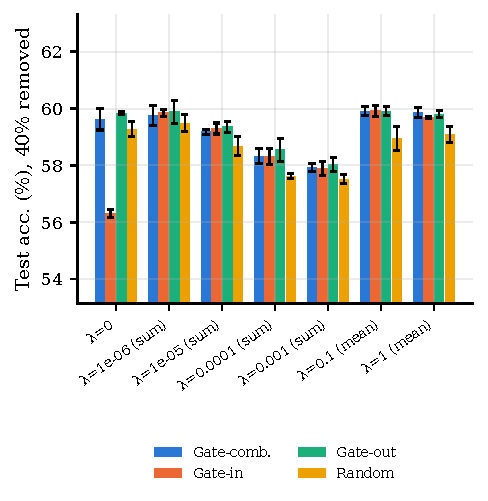
\includegraphics[width=\columnwidth]{mlp/fig_ablation_gate_lambda.pdf}
\caption{Ablation A: test accuracy after removing $40\%$ of hidden units from gated
sources trained with different penalties (mean $\pm$ SD, 3 seeds, 5 fine-tuning
epochs).}
\label{fig:lambda}
\end{figure}
